%==============================================================================
%  Measuring Muscle, Automatically -- 5 minute project presentation
%  CSE 754 Deep Learning for Computer Vision
%
%  Compile:  pdflatex main  (twice), or press Recompile on Overleaf.
%  Figures come from ../figures/, produced by scripts/make_figures.py and
%  scripts/make_result_figures.py.
%
%  Timing guide (10 content slides, roughly 30 s each):
%    1 title .......... 0:00      6 evaluation ...... 2:40
%    2 problem ........ 0:15      7 results ......... 3:10
%    3 the real task .. 0:45      8 what failed ..... 3:40
%    4 pipeline ....... 1:20      9 key finding ..... 4:10
%    5 calibration ..... 1:55     10 closing ......... 4:40
%==============================================================================

\documentclass[aspectratio=169,11pt]{beamer}

\usepackage[utf8]{inputenc}
\usepackage[T1]{fontenc}
\usepackage{graphicx}
\usepackage{booktabs}
\usepackage{amsmath}
\usepackage{tikz}
\usetikzlibrary{arrows.meta, positioning}

\usetheme{default}
\usecolortheme{default}
\setbeamertemplate{navigation symbols}{}
\setbeamertemplate{itemize items}[circle]

\definecolor{Ink}{HTML}{1D3557}
\definecolor{Accent}{HTML}{E07A1F}
\definecolor{Teal}{HTML}{2A9D8F}
\definecolor{Muted}{HTML}{5A7A9A}
\definecolor{Red}{HTML}{B3001B}

\setbeamercolor{frametitle}{bg=Ink, fg=white}
\setbeamercolor{title}{fg=Ink}
\setbeamercolor{structure}{fg=Ink}
\setbeamercolor{itemize item}{fg=Accent}
\setbeamercolor{itemize subitem}{fg=Teal}
\setbeamercolor{normal text}{fg=Ink}
\setbeamerfont{frametitle}{size=\large, series=\bfseries}
\setbeamerfont{footline}{size=\scriptsize}

% Frame title with an accent rule underneath.
\setbeamertemplate{frametitle}{%
  \nointerlineskip
  \begin{beamercolorbox}[wd=\paperwidth,ht=2.6ex,dp=1.3ex,leftskip=0.3cm]{frametitle}
    \usebeamerfont{frametitle}\insertframetitle
  \end{beamercolorbox}%
  \nointerlineskip
  \begin{beamercolorbox}[wd=\paperwidth,ht=0.35ex,dp=0ex]{}
    \hspace*{0.3cm}\textcolor{Accent}{\rule{0.28\paperwidth}{0.35ex}}
  \end{beamercolorbox}
}

\setbeamertemplate{footline}{%
  \hfill\textcolor{Muted}{\insertframenumber/\inserttotalframenumber}\hspace{0.35cm}\vspace{0.2cm}
}

\graphicspath{{figures/}{../figures/}}

\newcommand{\hl}[1]{\textcolor{Accent}{\textbf{#1}}}
\newcommand{\num}[1]{\textcolor{Ink}{\textbf{#1}}}

\title{Measuring Muscle, Automatically}
\subtitle{Geometry-aware deep learning for muscle architecture in B-mode ultrasound}
\author{Shamima Hossain \\ \small ID 21141119}
\institute{\small CSE 754 Deep Learning for Computer Vision}
\date{\small\today}

\begin{document}

%--------------------------------------------------------------------- 1 ----
\begin{frame}[plain]
  \vspace{0.8cm}
  \begin{center}
    {\Huge\bfseries\color{Ink} Measuring Muscle, Automatically\par}
    \vspace{0.4cm}
    {\large\color{Muted} Geometry-aware deep learning for muscle architecture\\
     estimation in B-mode ultrasound\par}
    \vspace{0.5cm}
    {\color{Accent}\rule{0.45\paperwidth}{1.2pt}}
    \vspace{0.5cm}

    {\large Shamima Hossain \quad\textcolor{Muted}{ID 21141119}\par}
    \vspace{0.2cm}
    {\color{Muted} CSE 754 Deep Learning for Computer Vision}
  \end{center}
\end{frame}

%--------------------------------------------------------------------- 2 ----
\begin{frame}{The problem}
  \begin{columns}[T]
  \begin{column}{0.53\textwidth}
    Three numbers describe muscle architecture:
    \begin{itemize}
      \item \hl{muscle thickness} (mm)
      \item \hl{pennation angle} (degrees)
      \item \hl{fascicle length} (mm)
    \end{itemize}
    \vspace{0.3cm}
    They are still measured \textbf{by hand}: slow, subjective, and dependent on
    operator experience.
    \vspace{0.3cm}

    \textbf{Goal.} Produce all three automatically from a single ultrasound
    frame.
  \end{column}
  \begin{column}{0.44\textwidth}
    \centering
    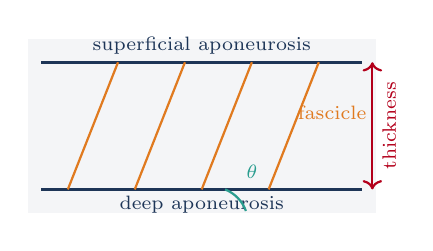
\begin{tikzpicture}[scale=0.85, every node/.style={font=\scriptsize}]
      \fill[Ink!5] (0,0) rectangle (5.2,2.6);
      \draw[Ink, very thick] (0.2,2.25) -- (5.0,2.25);
      \draw[Ink, very thick] (0.2,0.35) -- (5.0,0.35);
      \node[Ink] at (2.6,2.5) {superficial aponeurosis};
      \node[Ink] at (2.6,0.12) {deep aponeurosis};
      \foreach \x in {0.6,1.6,2.6,3.6} {
        \draw[Accent, thick] (\x,0.35) -- (\x+0.75,2.25);
      }
      \node[Accent] at (4.55,1.5) {fascicle};
      \draw[Teal, thick] (2.95,0.35) arc (68:20:0.55);
      \node[Teal] at (3.35,0.62) {$\theta$};
      \draw[Red, <->, thick] (5.15,0.35) -- (5.15,2.25);
      \node[Red, rotate=90] at (5.4,1.3) {thickness};
    \end{tikzpicture}
  \end{column}
  \end{columns}
\end{frame}

%--------------------------------------------------------------------- 3 ----
\begin{frame}{What the task actually is}
  The data does not make this a supervised regression problem.
  \vspace{0.35cm}

  \begin{columns}[T]
  \begin{column}{0.48\textwidth}
    \textbf{\color{Red} No measurement labels}\\[0.15cm]
    {\small Training data gives \emph{masks} only, never a thickness or an angle.
    The three targets must be \hl{reconstructed geometrically}.}
    \vspace{0.45cm}

    \textbf{\color{Red} No scale metadata}\\[0.15cm]
    {\small Two targets are in millimetres; the network sees pixels. The
    conversion must be \hl{read off the scanner's own depth ruler}.}
  \end{column}
  \begin{column}{0.48\textwidth}
    \textbf{\color{Red} Silent data defects}\\[0.15cm]
    {\small
    \begin{itemize}\setlength\itemsep{0.15cm}
      \item 70\% of frames disagree in size with their own mask
      \item 26\% of fascicle images are duplicates
    \end{itemize}
    Neither raises an error. Both corrupt results in ways that look like
    success.}
  \end{column}
  \end{columns}

  \vspace{0.4cm}
  \begin{center}
  \colorbox{Ink!8}{\parbox{0.92\textwidth}{\centering\small
  A naive split leaks \num{179} duplicate groups into validation.
  Content-grouped splitting reduces that to \num{0}.}}
  \end{center}
\end{frame}

%--------------------------------------------------------------------- 4 ----
\begin{frame}{Pipeline}
  \vspace{0.2cm}
  \centering
  \resizebox{\textwidth}{!}{%
  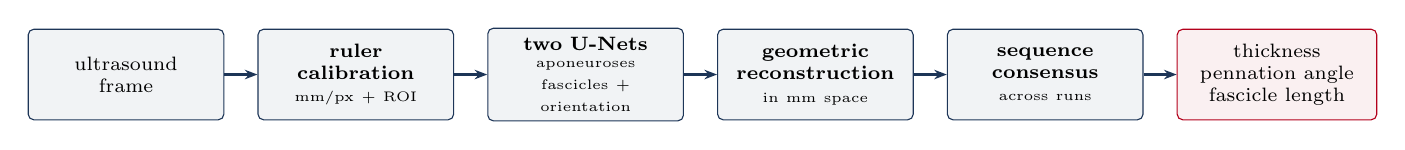
\begin{tikzpicture}[
      node distance=0.42cm,
      box/.style={draw=Ink, fill=Ink!6, rounded corners=2pt, minimum height=1.15cm,
                  text width=2.25cm, align=center, font=\scriptsize},
      result/.style={draw=Red, fill=Red!6, rounded corners=2pt, minimum height=1.15cm,
                  text width=2.3cm, align=center, font=\scriptsize},
      ar/.style={-{Stealth[length=1.6mm]}, Ink, thick}]

    \node[box] (in) {ultrasound\\frame};
    \node[box, right=of in] (cal) {\textbf{ruler}\\\textbf{calibration}\\\tiny mm/px + ROI};
    \node[box, right=of cal] (seg) {\textbf{two U-Nets}\\\tiny aponeuroses\\\tiny fascicles + orientation};
    \node[box, right=of seg] (geo) {\textbf{geometric}\\\textbf{reconstruction}\\\tiny in mm space};
    \node[box, right=of geo] (seq) {\textbf{sequence}\\\textbf{consensus}\\\tiny across runs};
    \node[result, right=of seq] (res) {thickness\\pennation angle\\fascicle length};

    \draw[ar] (in) -- (cal);
    \draw[ar] (cal) -- (seg);
    \draw[ar] (seg) -- (geo);
    \draw[ar] (geo) -- (seq);
    \draw[ar] (seq) -- (res);
  \end{tikzpicture}}

  \vspace{0.5cm}
  \begin{columns}[T]
  \begin{column}{0.31\textwidth}
    \centering{\footnotesize\textbf{Data}}\\[0.1cm]
    {\scriptsize
    1\,048 aponeurosis frames\\
    2\,761 fascicle frames\\
    309 unlabelled test frames}
  \end{column}
  \begin{column}{0.31\textwidth}
    \centering{\footnotesize\textbf{Model}}\\[0.1cm]
    {\scriptsize
    U-Net, ResNet-34 encoder\\
    512$\times$512, BCE + Dice\\
    94 min on one GPU}
  \end{column}
  \begin{column}{0.31\textwidth}
    \centering{\footnotesize\textbf{Contribution}}\\[0.1cm]
    {\scriptsize
    scale recovery\\
    dense orientation head\\
    geometry in mm space}
  \end{column}
  \end{columns}
\end{frame}

%--------------------------------------------------------------------- 5 ----
\begin{frame}{Scale calibration}
  \begin{columns}[T]
  \begin{column}{0.36\textwidth}
    {\small Six scanner families, each drawing its depth ruler differently:
    left edge, right edge, bottom edge; ticks every 5 or 10 mm.}
    \vspace{0.3cm}

    \begin{center}
    \colorbox{Teal!12}{\parbox{0.92\textwidth}{\centering
    \num{100\%} of the 309 test\\frames calibrate}}
    \end{center}
    \vspace{0.2cm}

    {\footnotesize Validated independently: implied field of view spans
    \num{2.97} to \num{6.95} cm deep, matching the documented
    3 to 7 cm scanner presets. Nothing was fitted to those numbers.}
  \end{column}
  \begin{column}{0.62\textwidth}
    \centering
    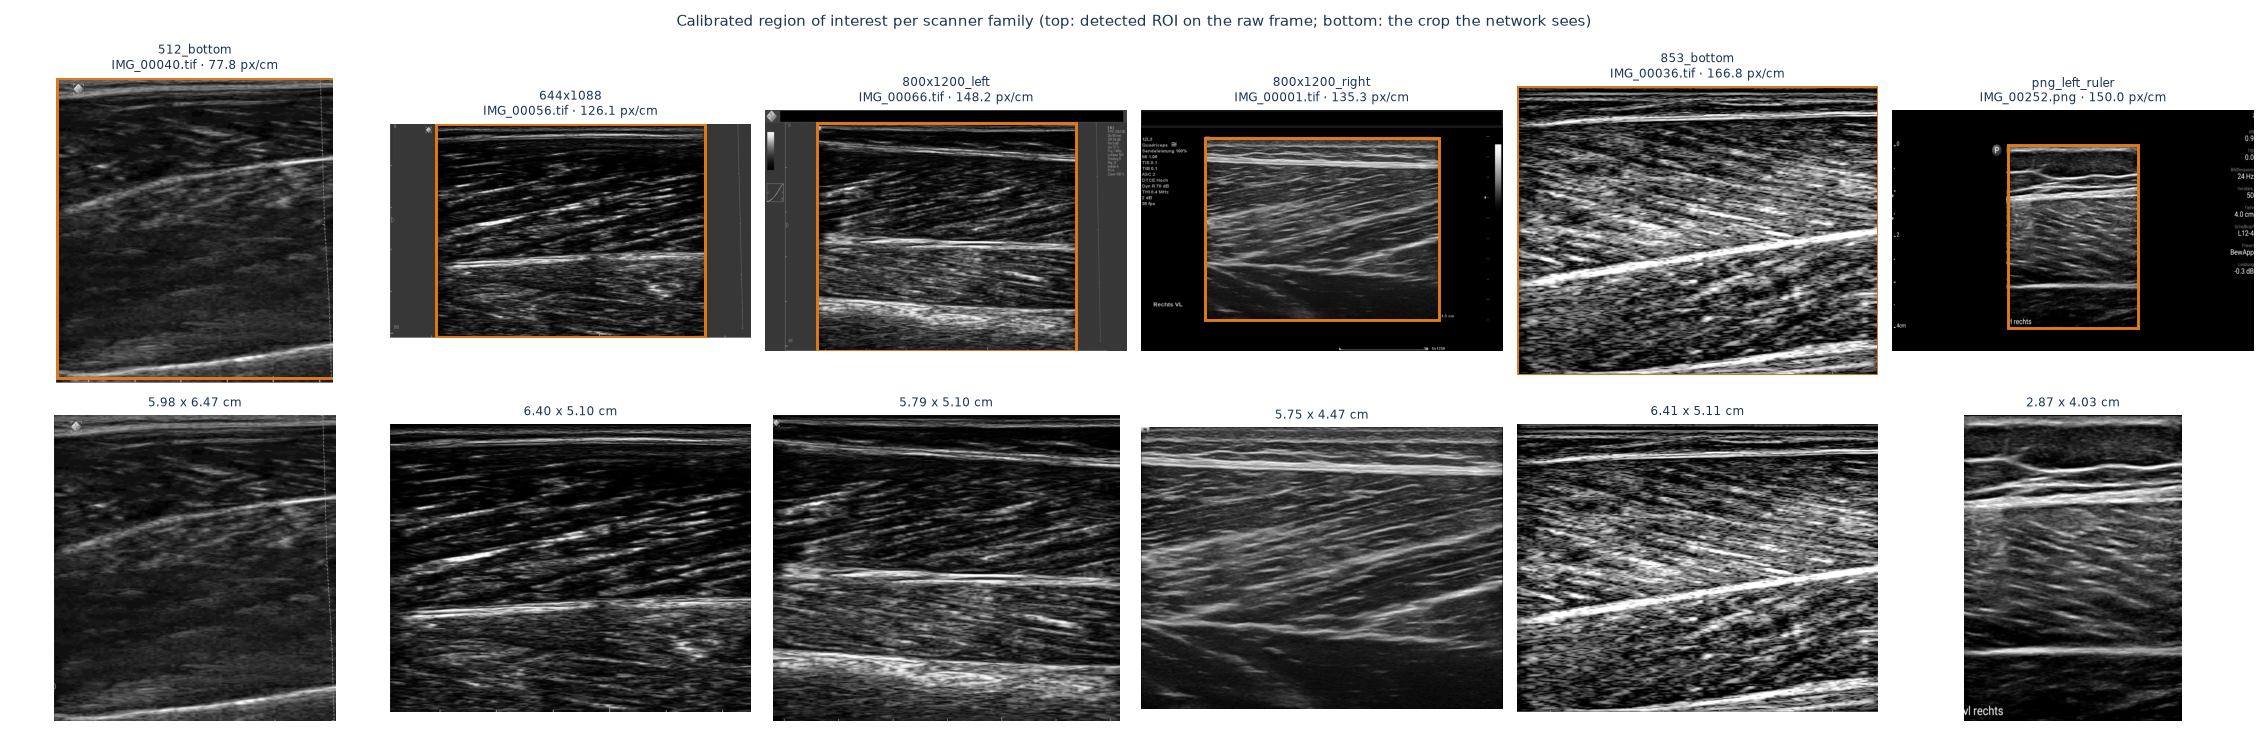
\includegraphics[width=\textwidth]{roi_by_family.png}\\[0.1cm]
    {\tiny Detected region of interest per scanner family, and the crop the
    network sees.}
  \end{column}
  \end{columns}
\end{frame}

%--------------------------------------------------------------------- 6 ----
\begin{frame}{Geometric reconstruction}
  \begin{columns}[T]
  \begin{column}{0.42\textwidth}
    {\small
    \begin{itemize}\setlength\itemsep{0.2cm}
      \item Aponeuroses fitted as \hl{curves}, not lines
      \item Pennation referenced to the \hl{deep aponeurosis}, as the clinical
            definition specifies
      \item Orientation predicted as a dense \hl{$(\cos 2\theta, \sin 2\theta)$
            field}, so that averaging directions is well defined
    \end{itemize}}
    \vspace{0.25cm}
    {\footnotesize Orientation targets are \emph{derived}, so they were checked
    against an independent estimator: median disagreement \num{1.1}
    degrees, 100\% of frames within 5 degrees.}
  \end{column}
  \begin{column}{0.56\textwidth}
    \centering
    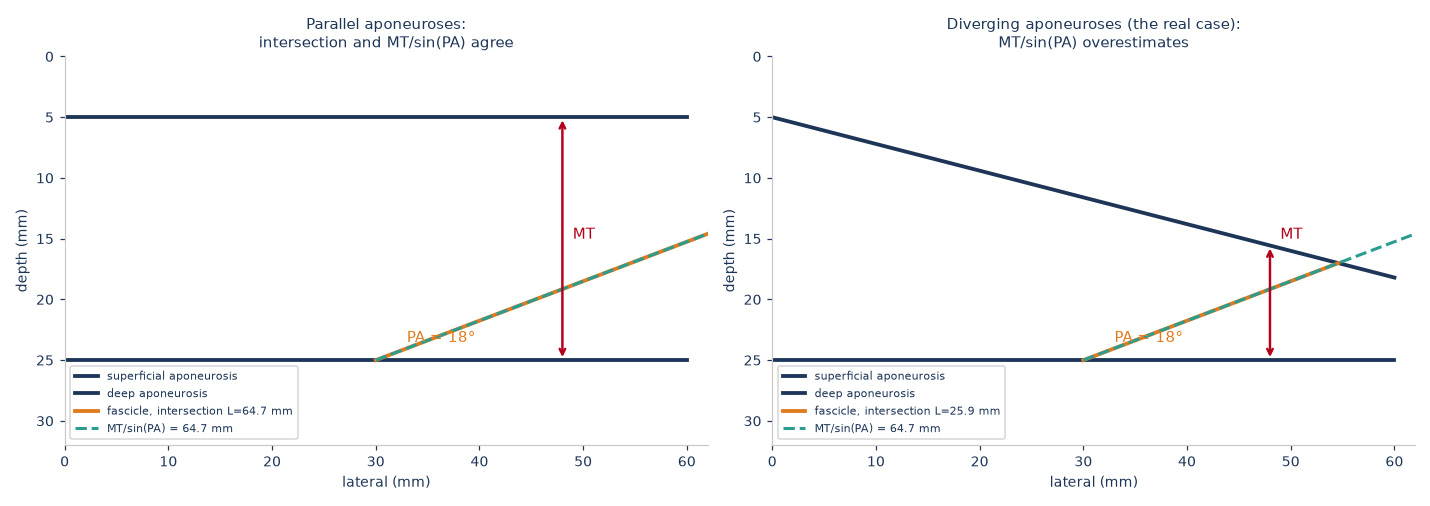
\includegraphics[width=\textwidth]{geometry_reconstruction.png}\\[0.15cm]
    {\tiny Two ways to reconstruct fascicle length. Which is better turned out
    to be the project's most interesting question.}
  \end{column}
  \end{columns}
\end{frame}

%--------------------------------------------------------------------- 7 ----
\begin{frame}{Evaluating without any measurement labels}
  No frame carries an expert measurement, so error against a human cannot be
  computed anywhere.
  \vspace{0.3cm}

  \begin{center}
  \colorbox{Ink!8}{\parbox{0.9\textwidth}{\centering
  \textbf{Pseudo-ground-truth protocol.} Run the \emph{same} geometry module
  twice, once on the annotator's masks and once on the network's, and compare.}}
  \end{center}
  \vspace{0.35cm}

  \begin{columns}[T]
  \begin{column}{0.48\textwidth}
    {\small\textbf{What it measures}\\
    the error the segmentation contributes, with the geometry held fixed.}
  \end{column}
  \begin{column}{0.48\textwidth}
    {\small\textbf{What it does not measure}\\
    error of the geometry module itself against a human. That needs expert
    annotations this data does not contain.}
  \end{column}
  \end{columns}
  \vspace{0.35cm}

  {\footnotesize \textbf{External check.} Pennation angle is scale-invariant, so
  the reconstruction run on annotator masks can be compared with the outside
  world without trusting the calibration: it gives a median of \num{17.0}
  degrees, against a published range of 10 to 25 degrees and \num{16.4} degrees
  for an independently built pipeline.}
\end{frame}

%--------------------------------------------------------------------- 8 ----
\begin{frame}{Results}
  \begin{columns}[T]
  \begin{column}{0.46\textwidth}
    {\small\textbf{Segmentation, held out}}\\[0.15cm]
    {\footnotesize
    \begin{tabular}{lrr}
      \toprule
       & aponeurosis & fascicle \\
      \midrule
      Dice & \textbf{0.839} & 0.274 \\
      IoU  & 0.731 & 0.161 \\
      Orientation & & \textbf{2.74\textdegree} \\
      \bottomrule
    \end{tabular}}
    \vspace{0.3cm}

    {\footnotesize The fascicle Dice is low because annotators traced a
    \emph{representative sample} of fascicles, not all of them. A model finding
    a different valid set is penalised while being correct for the purpose.}
  \end{column}
  \begin{column}{0.5\textwidth}
    {\small\textbf{Geometry, predicted vs annotator masks}}\\[0.15cm]
    {\footnotesize
    \begin{tabular}{lr}
      \toprule
      Muscle thickness & \textbf{0.3\% relative} \\
      Pennation angle  & \textbf{1.16\textdegree} \\
      Fascicle length  & 6.0\% relative \\
      \bottomrule
    \end{tabular}}
    \vspace{0.3cm}

    {\footnotesize Thickness is recovered from \emph{predicted} masks to within
    0.3\% of what the annotator's own masks give. That single fact drove the
    project's main design decision.}
    \vspace{0.2cm}

    {\scriptsize\color{Muted} Caveat: all 78 paired frames come from one scanner
    family.}
  \end{column}
  \end{columns}
\end{frame}

%--------------------------------------------------------------------- 9 ----
\begin{frame}{Ablations}
  \vspace{0.15cm}
  {\small
  \begin{tabular}{p{0.34\textwidth}p{0.6\textwidth}}
    \toprule
    \textbf{Proposed} & \textbf{Measured against what it replaced} \\
    \midrule
    Dense orientation head
      & \textcolor{Red}{Does not beat it.} 0.79\textdegree{} against
        \textbf{0.72\textdegree} for the classical structure tensor. \\[0.2cm]
    Sequence smoothing
      & \textcolor{Red}{Nearly inert.} Within-run spread was already
        0.02 mm in thickness. \\[0.2cm]
    Per-frame confidence
      & \textcolor{Red}{Does not predict error.} Spearman $-0.08$ to $-0.19$,
        not significant. \\[0.2cm]
    Intersection for fascicle length
      & \textcolor{Teal}{\textbf{Helps, but not for the proposed reason.}}
        See next slide. \\
    \bottomrule
  \end{tabular}}
  \vspace{0.3cm}

  {\footnotesize The confidence measure initially \emph{appeared} to detect
  failures. It was being told about them: an earlier version docked confidence
  whenever an estimate hit a clamp, so any correlation with error was circular.
  The term was removed.}
\end{frame}

%-------------------------------------------------------------------- 10 ----
\begin{frame}{The main finding}
  \begin{center}
  \colorbox{Accent!14}{\parbox{0.93\textwidth}{\centering
  \textbf{A model that is more faithful in principle can be a worse estimator
  in practice, when it depends on noisier inputs.}}}
  \end{center}
  \vspace{0.3cm}

  {\small The proposal argued that $\mathrm{FL} = \mathrm{MT}/\sin(\mathrm{PA})$
  is wrong because the aponeuroses are not parallel, and that intersecting the
  fascicle with the fitted curves is better. The premise is correct. The
  conclusion does not follow.}
  \vspace{0.25cm}

  \begin{columns}[T]
  \begin{column}{0.47\textwidth}
    {\footnotesize
    \begin{tabular}{lr}
      \toprule
      \textbf{Construction} & \textbf{Median error} \\
      \midrule
      Intersection & 0.077 \\
      Textbook $\mathrm{MT}/\sin(\mathrm{PA})$ & \textbf{0.060} \\
      \bottomrule
    \end{tabular}\\[0.15cm]
    Wilcoxon $p = 0.0003$, $n = 78$.}
  \end{column}
  \begin{column}{0.5\textwidth}
    {\footnotesize \textbf{Why.} Not because divergence is estimated badly: it
    is recovered to 0.15\textdegree. The textbook formula leans on
    \emph{thickness}, recovered to 0.3\%. The intersection leans on a
    \emph{difference of two fitted angles}, inheriting angular noise twice over.}
  \end{column}
  \end{columns}
  \vspace{0.25cm}

  {\footnotesize What the intersection actually contributes is
  \hl{boundedness}: it cannot diverge at shallow pennation, where
  $\mathrm{MT}/\sin(\mathrm{PA})$ runs away as $1/\sin$. Right mechanism, wrong
  reason.}
\end{frame}

%-------------------------------------------------------------------- 11 ----
\begin{frame}{Closing}
  \begin{columns}[T]
  \begin{column}{0.48\textwidth}
    {\small\textbf{What worked}}
    \begin{itemize}\setlength\itemsep{0.12cm}
      \item {\small Thickness to \num{0.3\%}, pennation to \num{1.16\textdegree}}
      \item {\small Aponeurosis Dice \num{0.839}}
      \item {\small Scale recovered on \num{100\%} of test frames}
    \end{itemize}
    \vspace{0.25cm}
    {\footnotesize The component that mattered most was \hl{scale recovery},
    which the original proposal never contemplated, because it assumed the
    measurements were learnable targets.}
  \end{column}
  \begin{column}{0.48\textwidth}
    {\small\textbf{Honest limitations}}
    \begin{itemize}\setlength\itemsep{0.12cm}
      \item {\small No expert-measurement validation anywhere}
      \item {\small Paired set is 78 frames from one scanner family}
      \item {\small Fascicle length is extrapolated, not observed}
      \item {\small Single split, single seed}
    \end{itemize}
  \end{column}
  \end{columns}
  \vspace{0.4cm}

  \begin{center}
  {\small\color{Muted}
  Code, report and full ablations:
  \texttt{github.com/silvererudite/umud-muscle-architecture}}
  \end{center}
\end{frame}

\end{document}
